\documentclass[letterpaper, twoside, 12pt]{memoir}
\usepackage{fontspec}

\setmainfont{Junicode}

\chapterstyle{ell}
\pagestyle{Ruled}

\title{{\HUGE Keeper's Call}\\
{\small Game Design Document}
\vspace{\fill} \\ 
Minstrelcy Studios
\vspace{\fill} \\ 
}
\author{J.R.~Omahen}

\begin{document}

\maketitle
\newpage

\tableofcontents

\chapter{Game Design}
\section{Summary}

A girl is wandering through the forest, playing near a lake. She hears a mysterious voice: a call, beckoning her to the water. There she discovers her true calling.

\section{Gameplay}

The player operates in first person, exploring the area surrounding the lake. The mysterious voice will beckon to the player, but the player won't know where it's coming from. The main obstacle to the player is a lack of familiarity with the environment, and not knowing where the voice is coming from. 

\section{Mindset}

The player should be intrigued, seeking to discover what the voice is, where it's coming from, and who it belongs to.

\chapter{Technical}
\section{Summary}

The game is a text-based adventure game (\textit{interactive fiction}), with very simple keyboard-based input. The target play time is \textbf{10---15 minutes}.

\section{Screens}

The opening screen will have an intro title, graphic, and note about the "help" option. The word "help" can be entered at any time to give the player the list of acceptable commands. The player will need to type "Start" when they are ready to begin. 

Each screen following will provide the player with a description of the area, including details about which directions are available to them. Finally, there will be a few areas where the player will "hear something," giving them the option to "listen." These scenes will be important story building points. 

\section{Controls}

Players will be able to enter the following inputs:
\\

\textbf{Directional}
\begin{itemize}
	\item Straight
	\item Left
	\item Right
	\item Turn around \\
\end{itemize} 

\textbf{Actions}
\begin{itemize}
	\item Listen
	\item Don't Listen
	\item Pick up \\
\end{itemize} 

\textbf{Support Menu}
\begin{itemize}
	\item Help
\end{itemize}

\section{Mechanics}
The game has two basic mechanics: \\

\textbf{Start -> Scene Description -> Direction input -> New Scene Description} \\

\textbf{Start -> Scene Description -> Action input -> Action Response -> Direction input -> New Scene Description}

\chapter{Level Design}

\begin{center}
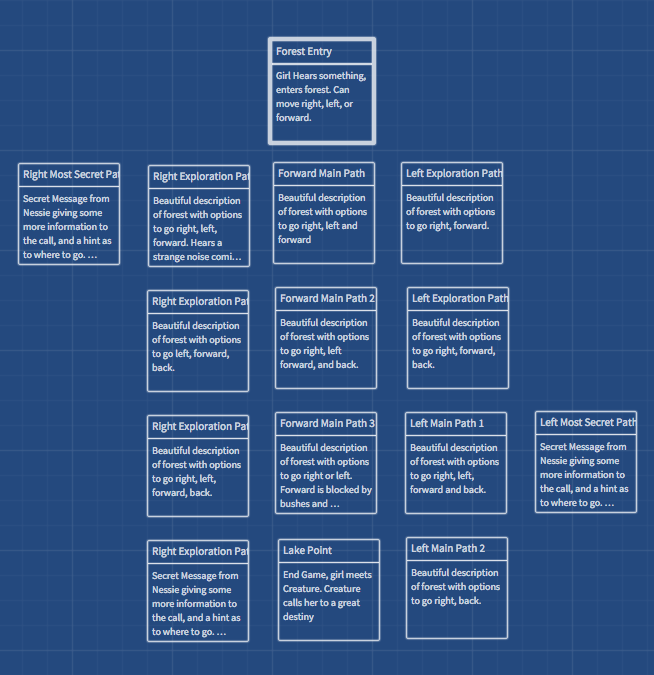
\includegraphics[scale=0.5]{Basic-Map-design.png}
\end{center}

\section{Themes}

\begin{enumerate}
\item Forest
\begin{itemize}
	\item Light Forest
	\begin{itemize}
		\item Light streams through branches
		\item Dark clouds above
		\item Tall trees
		\begin{itemize}
			\item Tall trunk
			\item Branches high up
			\item Light green leaves
		\end{itemize}
	\end{itemize}
\end{itemize}
\item Lake
\begin{itemize}
	\item Light green grass near the lake
	\item Ruined fortress near lake
	\item Deep Dark blue lake
	\begin{itemize}
		\item Still, beautiful
	\end{itemize}
	\item Light mist atop the lake
\end{itemize}
\end{enumerate}

\section{Game Flow}

\chapter{Development}
\section{Components}
\section{Component Compositions}

\chapter{Graphics}
\section{Style Attributes}
\chapter{Graphics Needed}

\chapter{Sound}
\section{Style Attributes}
\section{Sounds Needed}
\section{Music Needed}

\chapter{Development Timeline}

\chapter{Proposals}

\chapter{Rejected Ideas}


\end{document}